Figure \ref{fig:in_vitro_ex} shows a typical in vitro, epifluorescence data set (see Section \ref{sec:exp} for data collection details).  The top panel shows a field-of-view, including 3 neurons, two of which are patched.  To build our model, we first define a region-of-interest (ROI),  which is this case is the circled neuron.  Given the ROI, we can average all the pixel intensities of each frame, to get a one-dimensional fluorescence time-series, shown in the bottom left panel (black line).  Because we are patched onto this neuron, we also know when this neuron is spiking (black bars). 
Previous work suggests that this fluorescence signal might be well characterized by convolving the spike train with an exponential, and adding noise \cite{YusteKonnerth06}.  We confirmed that model for our data by convolving the true spike train with an exponential (gray line, bottom left panel), and then looking at the distribution of the residuals.  The bottom right panel shows (black line) a histogram of the residuals, and the best fit Gaussian distribution (gray line).


\begin{figure}[H]
\centering 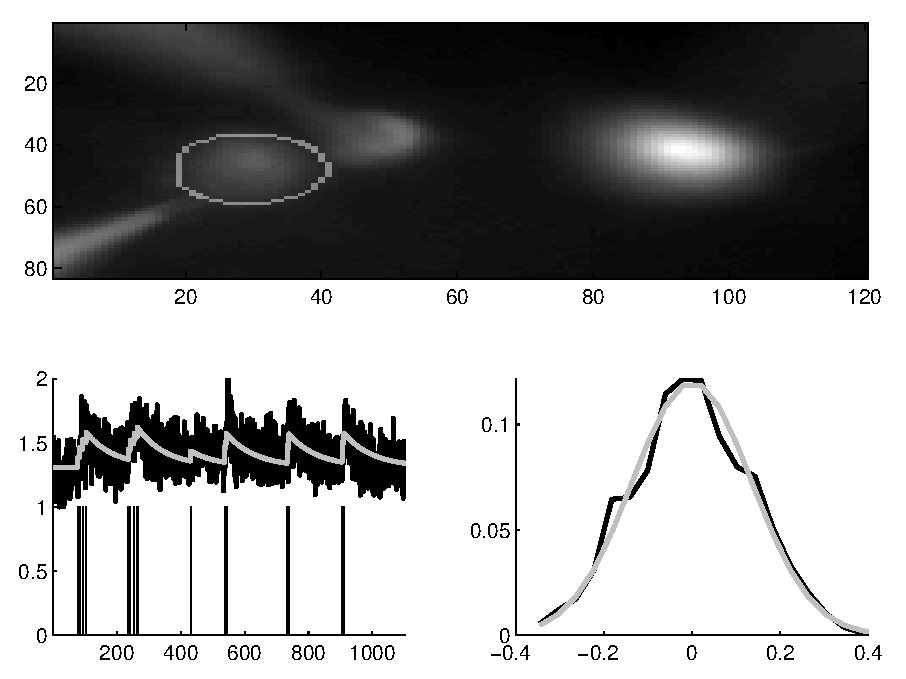
\includegraphics[width=.9\linewidth]{../figs/in_vitro_ex}
\caption{A typical in vitro data set suggests that a reasonable first order model may be constructed by convolving the spike train with an exponential, and adding Gaussian noise. Top panel: the average (over frames) of a typical field-of-view.  Bottom left: spike train (black bars), convolved with an exponential (gray line), superimposed on the one-dimensional fluorescence time series (black line).  Bottom right: a histogram of the residual error between the gray and black lines from the bottom left panel (black line), and the best fit Gaussian (gray line).} \label{fig:in_vitro_ex}
\end{figure}

The above observations may be formalized as follows. Assume we have a 1-dimensional fluorescence trace, $\bF=(F_1, \ldots, F_T)$ from a neuron.  At time $t$, the fluorescence measurement, $F_t$ is a linear-Gaussian function of the intracellular calcium concentration at that time, $C_t$:

\begin{align} \label{eq:F}
F_t &= \alpha (C_t + \beta) + \sig \varepsilon_t, \qquad \varepsilon_t \overset{iid}{\sim} \mN(0,1)
\end{align}

\noindent The scale, $\alpha$, absorbs all experimental variables impacting the scale of the signal, including number of sensors within the cell, photons per change in intracellular calcium concetration per sensor, amplification of imaging system, etc.  Similarly, the offset, $\beta$, absorbs baseline calcium concentration of the cell, background fluorescence of the fluorophore, imaging system offset, etc.  The standard deviation, $\sig$, results from calcium fluctuations independent of spiking activity, fluorescence fluctuations independent of calcium, and imaging noise. The noise at each time, $\varepsilon_t$, is independently and identically distributed according to a standard normal (i.e., Gaussian) distribution.  These three parameters, and the Gaussianity of the noise,  correspond to a number of simplifying assumptions, that we will relax in Section \ref{sec:results}.  

We further assume that the intracellular calcium concentration, $C_t$, jumps after each spike, and subsequently decays back down to rest with time constant, $\tau$, yielding:

% $\tau (C_t-C_{t-1})/\Del = -C_{t-1} + n_t$.  Rearranging (and rescaling) a bit, we have:

\begin{align} \label{eq:C}
\tau \frac{C_t - C_{t-1}}{\Del} &= - C_{t-1} + n_t
\end{align}

\noindent where $\Del$ is the time step size --- which in our case, is the frame duration, or $1/$(frame rate) --- and $n_t$ indicates the number of times the neuron spiked at time $t$. %, and $\gam=1-\Del/\tau$. \footnote{This follows from writing \eqref{eq:C} as $\tau \frac{C_t - C_{t-1}}{\Del} = -C_{t-1} + n_t$.} 
Note that $C_t$ does not refer to absolute intracellular concentration of calcium but rather, a relative measure.  The assumed linearity of our model precludes the possibility of determining calcium in absolute terms (but see Section \ref{sec:nonlin} for a modified model).  The gray line in the bottom left panel of Figure \ref{fig:in_vitro_ex} corresponds to the putative $\bC$ of the observed neuron.  

To complete the ``generative model'', we must also define the distribution from which spikes are sampled.  Perhaps the simplest first order description of spike trains is that at each time, spikes are sampled according to a Poisson distribution with some rate:

\begin{align} \label{eq:n}
	n_t \overset{iid}{\sim} \text{Poisson}(\lam \Del)
\end{align}

\noindent where $\lam \Del$ is the rate, and we have included $\Del$ to make $\lam$ be independent of the frame rate.  Thus, Eqs. \eqref{eq:F} -- \eqref{eq:n} complete our generative model.  


%Figure \ref{fig:schem} depicts a schematic illustration of this model. 

% \begin{figure}[H]
% \centering 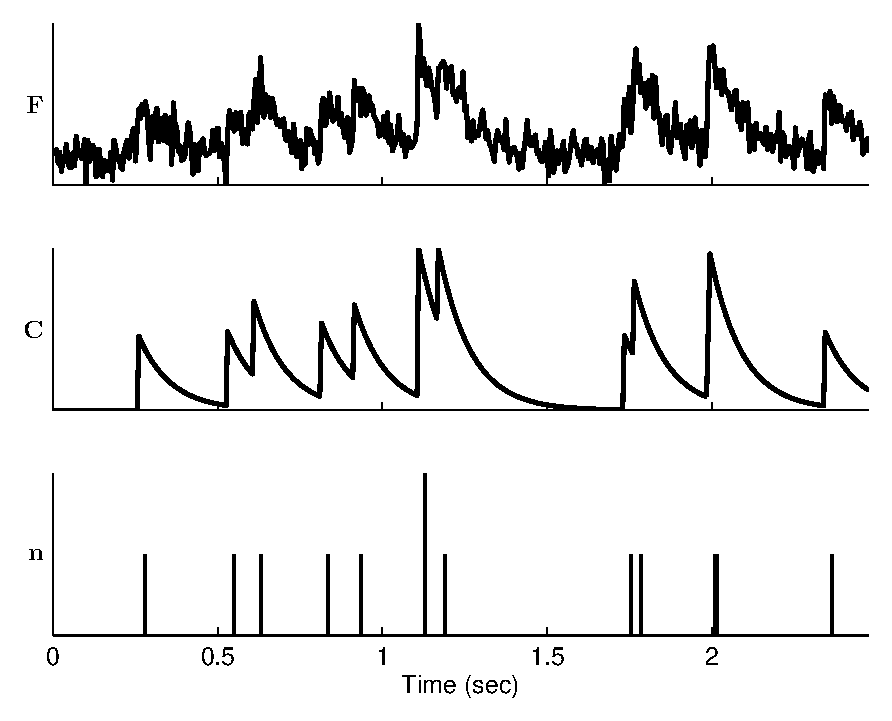
\includegraphics[width=.9\linewidth]{../figs/schem}
% \caption{A schematic illustrating our model. The spike train (bottom panel) is convolved with an exponential with time constant $\tau$ to obtain the calcium dynamics (middle panel).  The fluorescence observations are simply the calcium dynamics, plus zero mean Gaussian noise (with variance $\sig^2$). Parameters: $\Del=5$ msec, $\alpha=1$ photons/$\mu$M, $\beta=0$ unitless, $\sig=0.25$ photons, $\tau=100$ msec, $\lam=5$ Hz.} \label{fig:schem}
% \end{figure}


%relating spikes, $n_t$, baseline subtracted intracellular calcium concentration, denoted by $C_t$, and fluorescence measurements, $F_t$.  First, we assume a linear relationship between $F_t$ and $C_t$, with gaussian noise.  Second, we assume that $C_t$ jumps after each spike, and then decays according to some time constant.  Finally, we assume that spikes are distributed according to a Poisson process. The above assumptions lead to the follwoing model:

%. (1) spikes follow Poisson statistics with rate $\lam \Del$, (2) $C_t$ decays exponentially with decay $\gamma$ to baseline $\nu$, but jumps by $\rho$ after each spike, and (3) fluorescent observations are linear functions of $C_t$ with additive Gaussian noise with variance $\sig^2$.  Together, these assumptions imply the following model:

%\begin{align}
%\bF_t &= \balpha (C_t + \beta) +  \ve{\varepsilon}_t, \qquad &\ve{\varepsilon}_t \sim \mathcal{N}(\ve{0},\sig^2 \bI) \label{eq:obs} \\
%C_t  &= \gamma  C_{t-1} + n_t,  \qquad &n_t \sim \text{Poisson}(n_t; \lam \Del) \label{eq:trans}  
%\end{align}

%\noindent where $\balpha$ and $\beta$ set the fluorescence spatial filter and offset respectively, $\sig^2$ indicates the variance of the noise, and $\gamma$ sets the decay rate. 

%Note that   . To enforce identifiability, we will let $\balpha=1$ and $\beta=0$, without loss of generality, as explained below.


